Firstly, we discuss the feasibility of capturing a distribution via the \sindist{} -- i.e. we comment on the goodness of fit. Then we inspect the process of fitting the \sindist{} over multiple kinds of statistical objects -- Observational Likelihoods, Modal specifications, MSMs (moment summary measures), ECDFs and Discrete CDFs, and PDFs -- in an attempt to demonstrate its flexibility.


\section{MLE, Score equations}
The score equations for maximum likelihood estimation of the parameters of the \sindist{} $\Sinu(a,d,s,k)$ are not analytically solvable, as we detail below. Consider $X_i \iidsim \Sinu(a,d,s,k), \, i=1(1)n$. The likelihood will be given by 
\[L(a,d,s,k; \vector x) = \prod_{i=1}^n \indicator\set{a < x_i < a+d} \cdot \psi\left(\frac{x_i -a}{d}; s,k\right)\]
Putting the density expression and taking a logarithm, we get the joint log-likelihood as:
\begin{equation*}
    l(a,d,s,k; \utilde x)
    = \ln \indicator \set{x_{(1)}>a, \, x_{(n)}>a+d} -n\ln(d)-n\ln(A(s,k)) + k\sum_{i=1}^n \ln \sin \pi\left( x_i-a \over d \right)^s
\end{equation*}
Denote $z_i = \frac{x_i -a}{d}$. Some preliminary calculation:
\begin{align*}
    \nabla_s A &= \pi k \int_0^1 \sin^{k-1}(\pi z^s) \cos(\pi z^s) (\ln z) z^s \ \d z\\
    \nabla_k A &= \int_0^1 \sin^k(\pi z^s) \ln \sin(\pi z^s) \ \d z
\end{align*}
Gives us the score equations:
\begin{align*}
    &\nabla_a \ell = 0 \iff \sum_{i=1}^n z_i^{s-1} \cot(\pi z_i^s) = 0;  && \nabla_d \ell = 0 \iff \pi sk \sum_{i=1}^n z_i^s \cot(\pi z_i^s) = -n \\
    &\nabla_s \ell = 0 \iff  \pi k \sum_{i=1}^n {z^s \cos \pi z^s \ln z  \over \sin \pi z^s} = n {\nabla_s A \over A};  &&  \nabla_k \ell = 0 \iff \sum_{i=1}^n \ln \sin \pi z_i^s = n{\nabla_k A \over A}
\end{align*}
which may not be solved analytically. It may be wise to abandon this approach in favour of maximizing the joint likelihood through numerical computation means.

\section{Mode matching} \label{sec:modematch}
This method assumes that our target object has a unique, known mode and modal density, and that the support of the candidate \sindist{} is known or soundly estimable. WLoG, assume density is supported on $(0,1)$. Then, the remaining problem is only to optimize $s$ and $k$. Observe that $s,k$ jointly control the mode. So ``mode matching'', described as follows, presents one alternative to estimating $s,k$:
\begin{enumerate}
	\item Recall that the mode and the modal density of $\Sinu(s,k)$ are $2^{-1/s}$ and $1/A(s,k)$ respectively.
 	\item Equate $2^{-1/s} = \text{target mode}$. Call the solution $s^*$, tractable by analytical calculations alone.
	\item Equate $A(s^*, k) = \text{target modal density}$. Call the solution $k^*$, derivable by root-finding or optimization algorithms.
	\item Optimal candidate density is thus $\Sinu(s^*, k^*)$.
\end{enumerate}
It is to be noted that if this optimal density is a poor fit to the target, then either the target is not a Sinusoidal shape, or Sinusoidal distribution approximates is poorly within those bounds.

An example of usage of this method is demonstrated in \autoref{subsec:convolfit}.

\section{MSM on MSM}\label{sec:msmfit}
Given a set of 4 moment summary measures (MSMs), we focus on the problem of fitting to it an appropriate \sindist{} of 4 parameters, so that its MSMs match the specifications as closely as possible. For a given set of moment summary measures (MSMs) $\vec{\upmu}_0$, the MSM method hence minimizes w.r.t. $a,d,s,k$ the distance $L$ between the target MSMs and those of $\Sinu(a,d,s,k)$:
\[\min_{a,d,s,k} L(\vec{\upmu}_0 - \vec{\upmu}(a,d,s,k))\]
with a natural choice for $L$ being $\sum_{r=1}^4 (\upmu^0_r - \upmu_r(a,d,s,k))^2$.

Because $\Sinu(a,d,s,k)$ is a location-scale family in $(a,d)$, its first two MSMs (mean \& variance) can be freely adjusted by modifying $(a,d)$ alone, it should be sufficient to investigate the skewness-kurtosis adaptability of the distribution through its parameters $s$ and $k$. A numerical description of the skewness-kurtosis cover of the \sindist is provided in \autoref{fig:skewkurtcover}. Our optimization algorithm makes use of this fact by optimizing over $s, k$ jointly first, and then adjusting $a,d$ to meet the desired mean-variance requirements. A demonstration of this approach is presented in \autoref{fig:msmfit}.


\begin{figure}[h!]
	\centering
	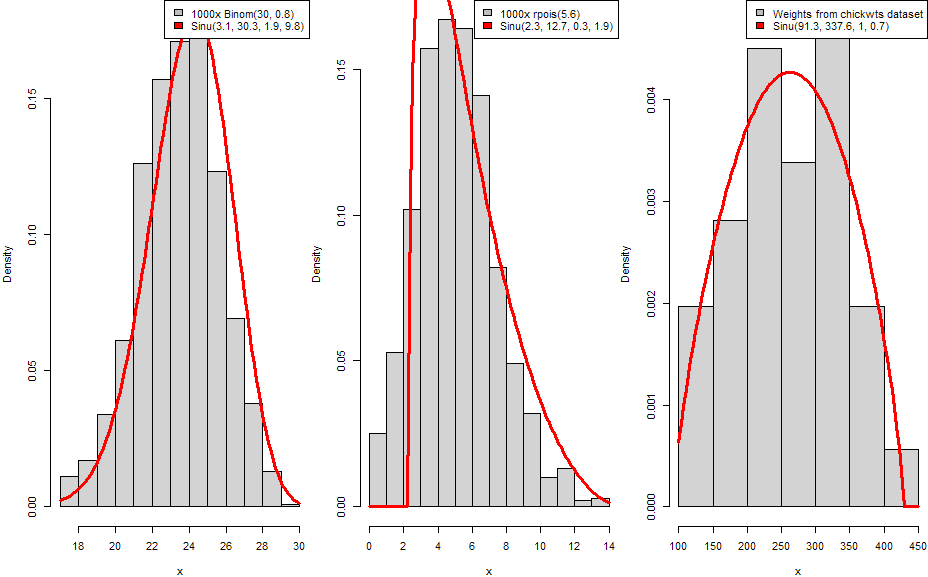
\includegraphics[width=0.8\linewidth]{fig/past/3-fitsinu-msm-hist}
	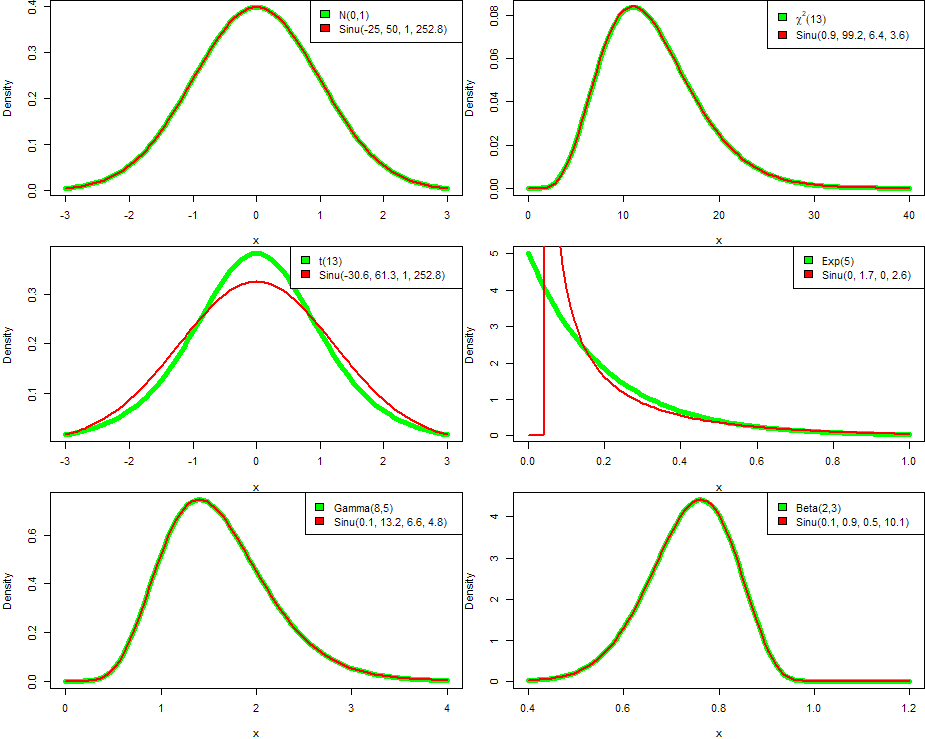
\includegraphics[width=0.8\linewidth]{fig/past/3-fitsinu-msm-curve}
	\caption{MSMs of $\Sinu(a,d,s,k)$ fitted over some theoretical and data MSMs.}
	\label{fig:msmfit}
\end{figure}

\section{PDF on PDF}
We tried fitting a $\Sinu(a,d,s,k)$ density over different target PDFs (standard location-scale members only) using numerical optimization (\texttt{L-BFGS-B} method of the \texttt{optim} function found in the \texttt{R} programming language) of a PDF-PDF divergence as follows:
\[\min_{a,d,s,k} L(f,g)\]
with a natural choice for $L$ being any density-density divergence metric, for example Hellinger metric $L(f,g) := \int_\mathscr{X} \frac 1 2 (\sqrt f-\sqrt g)^2 \d x$.
For finiteness of computation, we operated under the following parametric constraints whilst choosing the best candidate $\Sinu(a,d,s,k)$: $a \in [-10^3, 10^3]$, $d \in [10^{-2}, \, 2\times10^3]$, $s \in [10^{-2}, 10^2]$ and $k \in [10^{-2}, 10^2]$.
The results (minimized Hellinger distance with the choice of parameters) are provided in \autoref{tab:fitpdf}.
\begin{table}[h!]
    \centering
    \begin{tabularx}{\textwidth}{X|c}
        \toprule
        Target Density & Hellinger distance (Choice of Parameters $a,d,s,k$)\\
        \midrule
        $\N(0,1)$ & 0.00004277289 (-20.542932, 34.985498, 1.304535, 100)\\
        $\mathrm{Lognormal}(0,1)$ & 0.000936801 (0.02827762, 1000, 0.08566970, 35.78972) \\
        $\mathrm{Skew}\N_{\alpha=1} (0,1)$ & 2.189446e-05 (-7.2216216, 24.8516728, 0.5936823, 100) \\
        \hline
        $\mathrm{Logistic}(0,1)$ & 0.003149183 (-80.275639, 102.222513, 2.882431, 100) \\
        $\mathrm{Exp}(1)$ & 0.008101119 (0.0005708485, 6.5585684475, 0.0621246472, 1.6766166256) \\
        $\mathrm{DE}(0,1)$ & 0.01599712 (-8.895071, 16.872288, 1.085768, 15.608238) \\
        \hline
        $\Gamma(0.1,1)$ & Poor fit \\
        $\Gamma(100,1)$ & Poor fit \\
        $\Beta(1,1)$ & 0.0030202, (-0.0007780335, 1.0012066335, 0.1004892336, 0.12190192670) \\
        \hline
        $\mathrm{Cauchy}(0,1)$ & 0.06878475 (-126.211809, 149.303341, 4.141315, 100) \\
        \hline
        $\chi^2(1)$ & Poor fit \\
        $\chi^2(10)$ & 5.791378e-06 (-0.3201950, 97.1337699, 0.2815837, 22.0271292) \\
        $\mathrm{t}_1(0,1)$ & 0.06878477 (-126.114092, 149.207078, 4.138119, 100) \\
        $\mathrm{t}_{10}(0,1)$ & Fit failed \\
        $\mathrm{F}(1,1)$ & Poor fit \\
        \bottomrule
    \end{tabularx}
    \caption{Some common target densities and the best candidate \sindist{}}
    \label{tab:fitpdf}
\end{table}

The technical and theoretical underpinnings behind poor or failed fits will be the matter of future investigation.

\section{CDF on ECDF}\label{sec:cdffit}
We focus on the task of fitting a \sindist{} on a target ECDF $G_n$ by minimizing an $L_2$ loss of the following form:
\[\min_{a,d,s,k \in \Theta} L(F, G_n)^2\]
with a natural choice for $L$ being $\sum_{x \in X_i} (F-G_n)^2(x)$, where the summation is only over the observed datapoints. We choose such a metric primarily for its general finiteness and differentiability. Note that such techniques may seamlessly be used for discrete CDFs as well, by taking the summation over its masspoints instead.

The results of fitting some common CDFs/ECDFs are given in \autoref{fig:cdffit}.

\begin{figure}[h!]
	\centering
	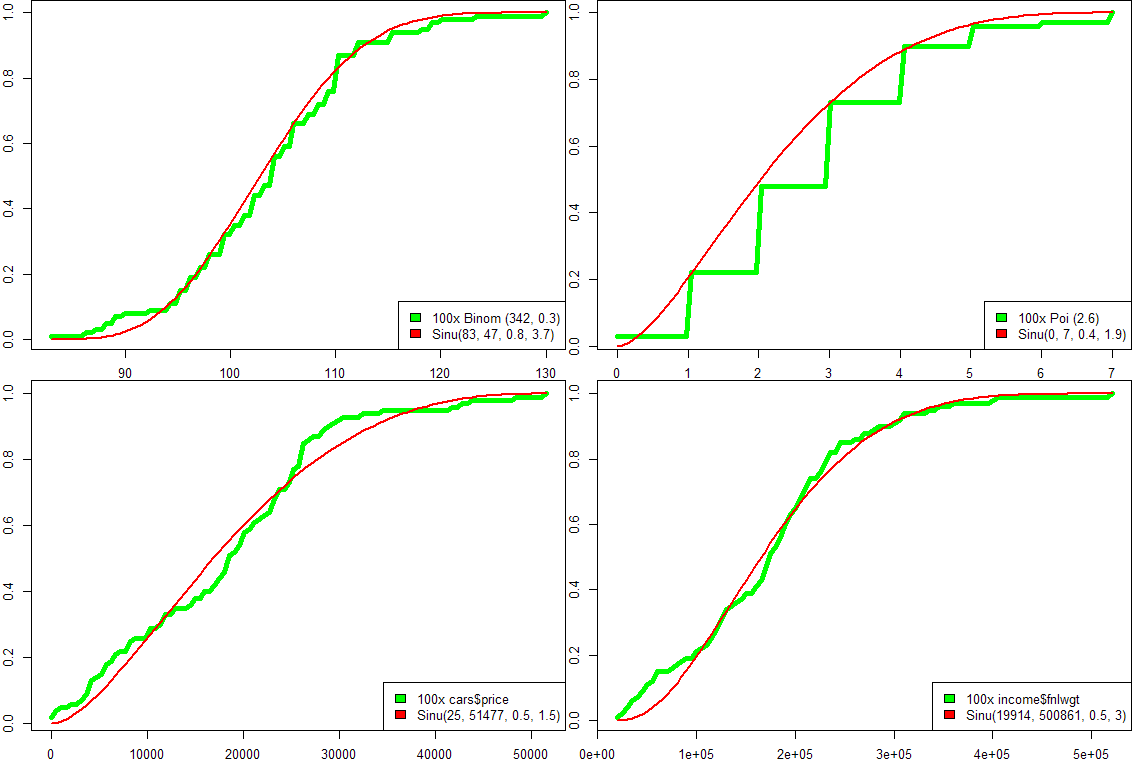
\includegraphics[width=0.8\linewidth]{fig/past/3-fitsinu-ecdf}
	\caption{CDF of $\Sinu(a,d,s,k)$ fitted over some theoretical and data ECDFs.}
	\label{fig:cdffit}
\end{figure}


\begin{comment}
	\section{QF on QF}
	Quantile function on Quantile Function
	
	\section{QF on EQF}
\end{comment}